Keyword spotting (KWS) has developed a lot over the years with one of the earliest approaches being based on the use of large-vocabulary continuos speech recognition (LVCSR) systems. An advantage to LVCSR-based KWS is its flexibility to deal with changing/non-predefined keywords. However, a big weakness to the LVCSR-based KWS is that it requires a large amount of computational resources, which can result in latency. This is an import factor when working with smaller online devices such as smartphones and smartwatches. A lighter alternative to LVCSR-based KWS is the keyword/filler hidden Markov model (HMM) approach. This approach trains a keyword HMM and a filler HMM to model keywords and non-keywords audio segments, respectively. Viterbi decoding is applied at runtime to find the optimal path in the decoding graph. Viterbi decoding can end up being computational demanding, depending on the topology of the HMM. The KWS system is then triggered whenever the likelihood ratio of the keyword model versus filler model is larger than a set threshold \cite{lopez2021deep}. 

Deep neural networks (DNN) have become very popular and are being used to develop new KWS systems. These systems are referred to as deep KWS systems and have become the new state of the art in KWS. Deep KWS systems do not need any complicated search algorithms like viterbi decoding, and they come with a huge improvement over the keyword/filler HMM approach in the case of low computational complexity \cite{lopez2021deep}. In general, deep KWS systems consist of three steps: speech features extraction, DNN acoustic model, and posterior handling, which is illustrated in \Cref{fig:deep_kws_system}.

\begin{figure}[h]
    \centering
    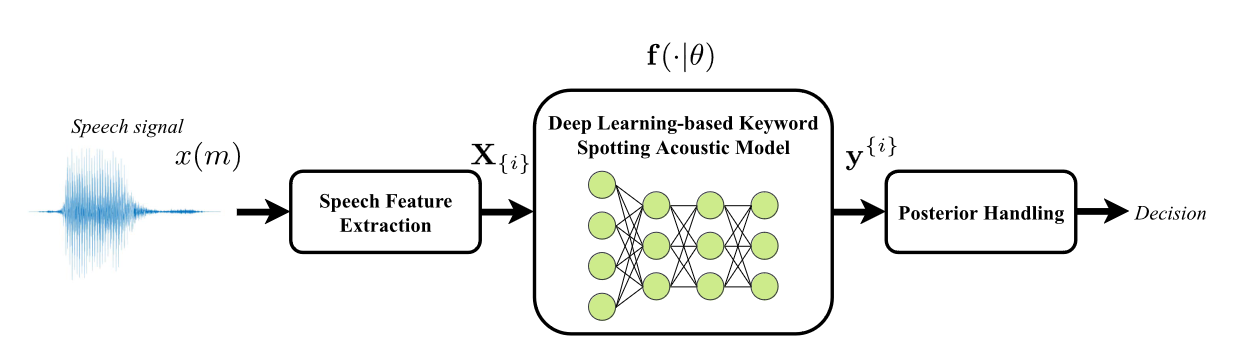
\includegraphics[width=\textwidth]{incl/img/kws/deep_kws_system.png}
    \caption{ Deep KWS system, from \cite{lopez2021deep}}
    \label{fig:deep_kws_system}
\end{figure}

\section{Speech Feature Extraction}
The speech feature extractor converts a speech signal, \(x(m)\), to a more compact representation of the speech. The speech features are often represented as a two dimensional matrix,
\begin{align}
    \textbf{X} = (\textbf{x}_0, \dots, \textbf{x}_{T-1}) \in \R^{K\times T},
\end{align}
where \(T\) is the amount of feature vectors, and \(K\) is the size of each feature vector. The amount of feature vectors depends on the length of the speech signal \cite{lopez2021deep}. 

Some of the popular speech features are the Mel-scale-related features. These could be the log-Mel spectral coefficients and Mel-frequency cepstral coefficients (MFCCs) \cite{lopez2021deep}. The common way to extract the log-Mel spectral and the MFCC features is shown on \Cref{fig:MFCC}. On the figure, it can be seen that to obtain the MFCC features you first have to get the log-Mel spectrogram coefficients, and then apply the discrete cosine transform to it. To stabilize and speed up the training of the DNN acoustic model, the features are normalized to a mean of zero and a standard deviation of one. This will also make the model more generalized \cite{lopez2021deep}. 

\begin{figure}[h]
    \centering
    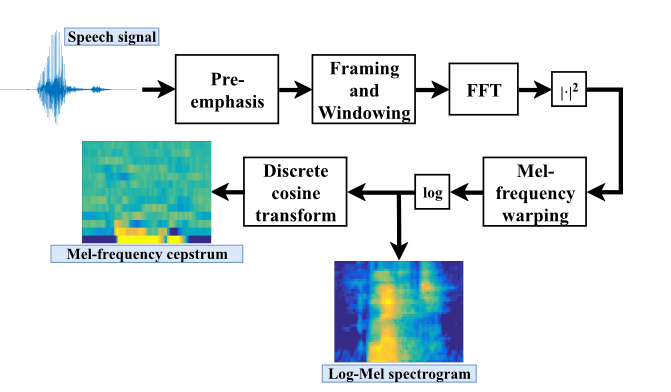
\includegraphics[width=\textwidth]{incl/img/kws/MFCC.png}
    \caption{ Classical pipeline for extracting log-Mel spectral and
    Mel-frequency cepstral speech features using the fast Fourier transform
    (FFT) \cite{lopez2021deep}}
    \label{fig:MFCC}
\end{figure}


\section{DNN KWS acoustic model}
The output of the speech feature extraction \(\textbf{X}\) is fed to the DNN acoustic model, which then outputs a sequence of probabilities, one for each keyword and non-keyword class. The way the acoustic model go through \(\textbf{X}\) is by taking a smaller section at a time, each section given as
\begin{align}
    \textbf{X}_{\{i\}} = \qty(\textbf{x}_{is-P}, \dots, \textbf{x}_{is}, \dots, \textbf{x}_{is+F}) \in \R^{K\times (P+F+1)},
\end{align} 
where \(i = \lceil \frac{P}{s} \rceil, \dots, \lfloor \frac{T-1-F}{s} \rfloor\) is a segment, \(s\) represents the time shift i.e., the overlap, \(P\) is the number of past frames, and \(F\) the number of future frames. Two examples of consecutive sections are illustrated on \Cref{fig:acoustic_model}. 

Denoting the DNN acoustic model as 
\begin{align}
    \textbf{f}\qty(\cdot|\theta): \R^{K\times (P+F+1)} \rightarrow I^N, 
\end{align}
where \(\theta\) is the input of the model, \(I = [0,1]\), and \(N\) the number of classes, we get the output probabilities, \(\textbf{y}^{\{i\}}\), of the model, given a segment \(\textbf{X}_{\{i\}}\),
\begin{align}
    \textbf{y}_n^{\{i\}} = \textbf{f}_n\qty(\textbf{X}_{\{i\}}|\theta), \quad n = 1, \dots, N,
\end{align}
where \(n\) denotes the \(n\)'th element of a vector. Denoting \(C_n\) as the \(n\)'th class we get that \(\textbf{y}_n^{\{i\}} = P(C_n|\textbf{X}_{\{i\}}, \theta)\) is the probability of \(\textbf{X}_{\{i\}}\) belonging to \(C_n\). To ensure that \(\textbf{y}_n^{\{i\}}\) is a probability, i.e., 
\begin{align}
    \sum_{n=1}^N \textbf{y}_n^{\{i\}} = 1 \quad \forall \ i,
\end{align}
a softmax activation function \cite{rothman2020artificial} is commonly used on the last layer \cite{lopez2021deep}.

\begin{figure}[h]
    \centering
    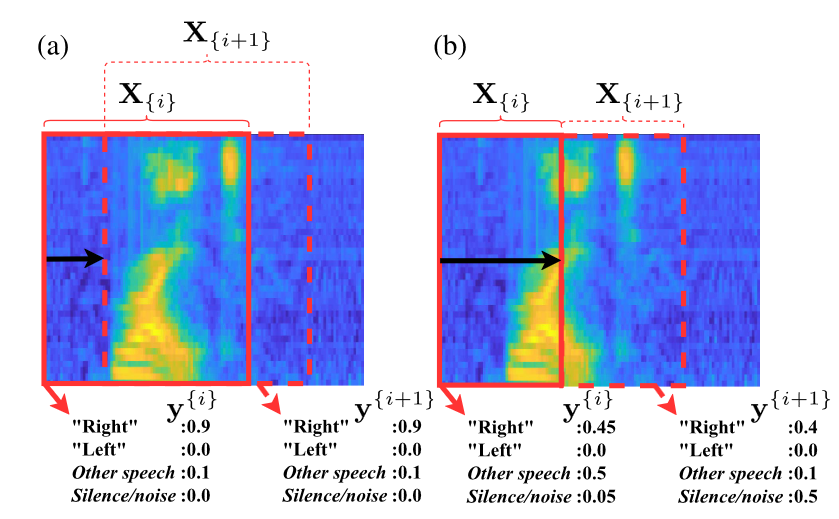
\includegraphics[width=\textwidth]{incl/img/kws/acoustic_model.png}
    \caption{Example of the processing of two consecutive feature segments \(\textbf{X}_{\{i\}}\) and \(\textbf{X}_{\{i +1\}}\), from \(\textbf{X}\) comprising the keyword "right", by a DNN acoustic model: (a) when using an overlapping segmentation window, and (b) when using a smaller, non-overlapping one \cite{lopez2021deep}. }
    \label{fig:acoustic_model}
\end{figure}

To pick which class a certain segment belongs to, one could just pick the class with highest probability, which could lead to different errors. Two cases where this approach will fail are shown in \Cref{fig:acoustic_model}, where an overlapping segment window is used on (a), and a smaller non-overlapping segment is used on (b). In the case of (a) the word "right" is found twice leading to a false positive detection and in the case of (b), "right" is not found a single time, leading to a false negative. This is one of the reasons why a good posterior handling is needed \cite{lopez2021deep}.

\subsection{Transformer Models}
The keyword transformer 

The KWT model is based on a vision transformer \cite{dosovitskiy2020image}, where the image is substituted with Mel-frequency cepstral coefficients (MFCC), which are explained in \Cref{ch:theory}, and have achieved state-of-the-art performance on the Google Speech Commands KWS benchmark.

\section{Posterior Handling}
To get a good final decision of class, the sequence of probabilities, \(\textbf{y}^{\{i\}}\), needs to be processed. There are two main modes when applying posterior handling: non-streaming and streaming modes.

\textbf{Non-streaming mode} is the simpler of the two, it is a standard multi-class classification of independent input segments. Since it only works on one segment, the segment needs to be long enough to contain a whole word – this could be around one second. \cite{lopez2021deep}. Posterior handling, in this mode, is the straight forward method of picking the class with the highest probability. This is not a very realistic method, because KWS in not a static task \cite{lopez2021deep}.

\textbf{Streaming mode} is, on the other hand, when the processing happens continuously, and normally in real-time \cite{lopez2021deep}. In this mode, the output sequence of probabilities from the acoustic model
\begin{align}
    \qty\{ \dots, \textbf{y}^{\{i-1\}}, \textbf{y}^{\{i\}}, \textbf{y}^{\{i+1\}}, \dots\},
\end{align}
is typically smoothened over time, classically a moving average is used. The smoothed probabilities, \(\bar{\textbf{y}}^{\{i\}}\), are often used to determine the keyword, or the lack of one. This is done either by comparing them with a sensitive threshold or by picking the class with the highest probability within a time sliding window. In the case of two consecutive segments covering the same keyword, a simple method is implemented, where all spotted keywords are ignored for a short period of time right after a keyword is spotted.

